% This is samplepaper.tex, a sample chapter demonstrating the
% LLNCS macro package for Springer Computer Science proceedings;
% Version 2.20 of 2017/10/04
%
\documentclass[runningheads]{llncs}
%
\usepackage{caption}  % For custom captions\usepackage{cite}     % For handling citations
\usepackage{amsmath}  % For mathematical features
\usepackage{graphicx}
\usepackage{booktabs}

\usepackage[colorlinks=true, urlcolor=blue, linkcolor=black]{hyperref}
% Used for displaying a sample figure. If possible, figure files should
% be included in EPS format.
%
% If you use the hyperref package, please uncomment the following line
% to display URLs in blue roman font according to Springer's eBook style:
% \renewcommand\UrlFont{\color{blue}\rmfamily}



\begin{document}
%
\title{Stroke Prediction Capstone Project}
%
%\titlerunning{Abbreviated paper title}
% If the paper title is too long for the running head, you can set
% an abbreviated paper title here
%
\author{Alvaro Quintero Gonzalez}
%
\authorrunning{A. Quintero Gonzalez.}
% First names are abbreviated in the running head.
% If there are more than two authors, 'et al.' is used.
%
\institute{Northwest Missouri State University, Maryville MO 64468, USA \\
\email{S573928@nwmissouri.edu and alvaroquintero28@yahoo.com}\\
}
%
\maketitle              % typeset the header of the contribution
%
\begin{abstract}
Stroke prediction is a critical area of research in healthcare, aiming to enhance preventative strategies and improve patient outcomes. This study investigates a comprehensive dataset collected from various healthcare sources, consisting of demographic, clinical, and lifestyle factors associated with stroke risk. The dataset encompasses attributes such as age, gender, blood pressure, cholesterol levels, body mass index (BMI), and lifestyle habits. "will finish at completion"

\keywords{Stroke Prediction \and Preventative Strategies \and Demographic Factors \and Predictive Modeling \and Machine Learning Algorithms}
\end{abstract}
%
%
%
\section{Introduction}

Strokes are a major health concern globally, recognized as one of the leading causes of disability and death. Occurring when blood flow to the brain is disrupted, it can lead to significant physical, cognitive, and emotional impairments in affected individuals. \cite{kaur2022retracted} The impact of strokes extends beyond the individual, affecting families and communities, and placing a substantial strain on healthcare systems. With the rising incidence of strokes associated with aging populations and the increasing prevalence of risk factors such as hypertension, obesity, and diabetes, there is an urgent need to focus on effective stroke prevention strategies. Prevention requires a multifaceted approach that includes public education, early identification of risk factors, and lifestyle modifications. Simple changes, such as adopting a balanced diet, engaging in regular physical activity, and managing underlying health conditions, can greatly reduce an individual's risk of stroke.\cite{doi:10.1161/STR.0000000000000375} Moreover, healthcare providers must play an active role in raising awareness about stroke prevention and ensuring that at-risk patients receive appropriate screenings and interventions. By promoting a comprehensive understanding of stroke risk factors, we can empower individuals to take charge of their health. This proactive approach not only aims to reduce the frequency of strokes but also facilitates overall public health awareness, fostering healthier communities. As advances in knowledge and strategies for stroke prevention, we can work towards a future where strokes are less frequent and their consequences are minimized \cite{sirisha2021awareness}.

\subsection{Define the Problem and Goals of This Capstone Project} 
This section discusses the goals of the proposed project. The primary focus of this capstone project is to develop a comprehensive understanding of stroke prediction and prevention strategies using data-driven approaches. Main goal consist of identifying key risk factors. By applying statistical analysis and machine learning techniques, it will determine which variables are most predictive of stroke occurrence. Further focus will evaluate performance of developed models in predicting stroke events, thereby providing valuable insights for early intervention. The project will propose targeted preventive strategies that can be implemented in community health programs therefore enhancing greater public awareness.

\subsubsection*{Project Links}
Key resources for this project provided below:

\begin{itemize}
    \item \href{https://github.com/alvaroquintero28/Capstone-Project-Report}{Capstone-Project-Report GitHub}
    \item \href{https://es.overleaf.com/read/zqgzcfntnwbz#9bc8ce}
    {Capstone Project Report Overleaf}
\end{itemize}

\subsection{The following are the phases of project implementation}

\begin{enumerate}
    \item Define the Problem and Objectives
    \begin{enumerate}
        \item Clearly articulate the specific questions and objectives of the analysis, focusing on how heart disease predictions can improve preventive measures for stroke patients.
         \item Identify key performance indicators (KPIs) to measure the success of the project. 
\end{enumerate}
\item  Literature Review and Background Research
\begin{enumerate}
    \item Conduct a thorough review of existing literature on heart disease, stroke rehabilitation, and predictive analytics in healthcare. 
    \item Gather insights into current best practices and identify gaps in the existing research that your project can address. 
\end{enumerate}
\item Data Collection
\begin{enumerate}
    \item Search for relevant datasets using the identified sources (e.g., ProjectPro, American Journal of Medicine) focusing on: 
    \begin{enumerate}
        \item Patient demographics 
        \item Medical history related to heart disease and strokes 
        \item Lifestyle factors (e.g., diet, exercise) 
        \item Laboratory test results (e.g., cholesterol levels, blood pressure) 
    \end{enumerate}
    \item Ensure that the data is reliable, accurate, and representative of the population you wish to study. 
\end{enumerate}
\item Data Pre-processing
    \begin{enumerate}
        \item Clean the data by handling missing values, outliers, and inconsistencies. 
        \item Perform data normalization or standardization if necessary. 
        \item Encode categorical variables to facilitate analysis in machine learning models. 
    \end {enumerate}
\item  Exploratory Data Analysis (EDA)
    \begin{enumerate}
        \item Analyze the dataset to uncover patterns and relationships between variables. 
        \item Use visualizations (graphs, plots) to represent findings and identify key risk factors associated with heart disease in stroke patients. 
    \end{enumerate}
\item Feature Selection
\begin{enumerate}
    \item Identify and select the most relevant features that influence heart disease predictions. 
    \item Use techniques like correlation analysis, recursive feature elimination (RFE), or machine learning algorithms to enhance feature selection. 
\end{enumerate}
\item Model Development
    \begin{enumerate}
        \item Choose appropriate machine learning models for prediction, such as: 
            \begin{enumerate}
                \item \item Logistic Regression
                \item Decision Trees 
                \item Random Forest 
                \item Support Vector Machines 
                \item Neural Networks 
            \end{enumerate}
        \item Split the dataset into training and testing sets for model evaluation. 
    \end{enumerate}
\item Model Training and Tuning
    \begin{enumerate}
        \item Train the selected models on the training dataset. 
        \item Optimize model performance using techniques like hyperparameter tuning and cross-validation to prevent overfitting. 
    \end{enumerate}
\item Model Evaluation
\begin{enumerate}
    \item Assess the accuracy and effectiveness of the models using the testing dataset. 
    \item Use evaluation metrics such as accuracy, precision, recall, F1 score, and the ROC-AUC curve to measure performance. 
    \item Compare the performance of different models to select the best one. 
\end{enumerate}
\item Conclusion
\begin{enumerate}
    \item Interpret Results
        \begin{enumerate}
            \item Analyze the results of the best-performing model to understand the impact of various factors on heart disease predictions. 
            \item Provide actionable insights and recommendations for preventing heart disease in stroke patients based on the findings. 
        \end{enumerate}
\item Discussion of the limitations
\item Ideas for future work.
\end{enumerate}

\section{Literature Review and Background Research}
Numerous studies have identified effective preventive measures for reducing the risk of stroke, emphasizing both management of hypertension and lifestyle interventions. \cite{sirisha2021awareness} Hypertension is the most significant modifiable risk factor for stroke, and studies have shown that controlling blood pressure through lifestyle changes, such as a healthy diet, regular physical activity, reducing sodium intake, smoking cessation, and adhering to prescribed antihypertensive medications can significantly lower the likelihood of experiencing a stroke. Maintaining blood pressure within a normal range (typically less than 120/80 mmHg) is crucial in preventing both ischemic and hemorrhagic strokes, making it the most critical focus in stroke prevention efforts. \cite{doi:10.1161/STR.0000000000000375} Combined, these research findings underscore the importance of a multifaceted approach to stroke prevention that integrates medical treatment with proactive lifestyle changes.

\subsection{Limitations}
The healthcare stroke prevention dataset and the well-being and lifestyle dataset each have inherent limitations that may affect the comprehensiveness and applicability of their findings. Firstly, the stroke prevention dataset may suffer from issues related to sample size and demographic representation, potentially limiting the generalizability of the results across diverse populations. Additionally, the accuracy of self-reported data regarding lifestyle factors in the well-being and lifestyle dataset may be compromised by social desirability bias, where participants might under-report unhealthy behaviors or exaggerate healthy ones. Furthermore, the transient nature of lifestyle habits makes it challenging to capture accurate and stable data over time, potentially leading to discrepancies in understanding long-term behavior trends.

\section{Data}
Data collection for this analysis involved two comprehensive datasets sourced from Kaggle: the Wellbeing and Lifestyle Data and the Healthcare Dataset on Stroke Data. The Wellbeing and Lifestyle Data dataset encompasses a variety of factors influencing individual health and well-being, such as lifestyle choices. It features demographic information, including age, gender, and socioeconomic status, facilitating an understanding of how these variables correlate with reported well-being outcomes. The Healthcare Dataset and Stroke Data, on the other hand, presents critical health metrics and conditions related to stroke incidents among patients. By merging insights from these two datasets, a more comprehensive picture of lifestyle influences on health outcomes can be constructed, enabling a deeper exploration of the relationships between well-being, lifestyle choices, and stroke risk.


\subsection{Dataset Variable Attributes}

The following tables summarize the original data attributes, including their descriptions, data types, and possible values prior to any data cleaning. These attributes are essential for understanding the collected data and are crucial for any subsequent analysis.

\clearpage
\begin{table}[ht]
\centering
\caption{Attributes, Descriptions, and Possible Values from Healthcare Dataset}
\label{tab:healthcare_data_attributes}
\begin{tabular}{|l|p{5cm}|p{4cm}|}
\hline
\textbf{Attribute} & \textbf{Description} & \textbf{Possible Values} \\ 
\hline
\textbf{id} & Unique identifier for each patient & Whole numbers \\ 
\hline
\textbf{gender} & Gender of the patient & "Male", "Female", "Other" \\ 
\hline
\textbf{age} & Age of the patient in years & Whole numbers (e.g., 0, 1, 25, 60) \\ 
\hline
\textbf{hypertension} & Indicates if the patient has hypertension & 0 (No), 1 (Yes) \\ 
\hline
\textbf{heart\_disease} & Indicates if the patient has heart disease & 0 (No), 1 (Yes) \\ 
\hline
\textbf{ever\_married} & Indicates if the patient has ever been married & "Yes", "No" \\ 
\hline
\textbf{work\_type} & Type of employment of the patient & "Children", "Govt job", "Self-employed", "Private", "Never worked" \\ 
\hline
\textbf{Residence\_type} & Type of residence of the patient & "Urban", "Rural" \\ 
\hline
\textbf{avg\_glucose\_level} & Average glucose level of the patient & Positive floats (e.g., 70.0, 220.0) \\ 
\hline
\textbf{bmi} & Body Mass Index of the patient & Positive floats (e.g., 18.5, 30.0) or "N/A" \\ 
\hline
\textbf{smoking\_status} & Indicates the smoking status of the patient & "formerly smoked", "smokes", "never smoked", "Unknown" \\ 
\hline
\textbf{stroke} & Indicates if the patient has had a stroke & 0 (No), 1 (Yes) \\ 
\hline
\end{tabular}
\end{table}

\clearpage

\begin{table}[ht]
\centering
\caption{Attributes, Descriptions, and Possible Values from Work-Life Balance Dataset}
\label{tab:work_life_balance_attributes}
\begin{tabular}{|l|p{5cm}|p{4cm}|}
\hline
\textbf{Attribute} & \textbf{Description} & \textbf{Possible Values} \\ 
\hline
\textbf{Timestamp} & Date of the record entry & Date format (e.g., "7/7/15") \\ 
\hline
\textbf{FRUITS\_VEGGIES} & Number of servings of fruits and vegetables consumed daily & Whole numbers (e.g., 0, 1, 2, 10) \\ 
\hline
\textbf{DAILY\_STRESS} & Daily stress level rating & Whole numbers (e.g., 1 to 10) \\ 
\hline
\textbf{PLACES\_VISITED} & Number of places visited daily & Whole numbers (e.g., 0, 1, 2, 10) \\ 
\hline
\textbf{CORE\_CIRCLE} & Number of close relationships or friends & Whole numbers (e.g., 0, 1, 8) \\ 
\hline
\textbf{SUPPORTING\_OTHERS} & Amount of time spent supporting others & Whole numbers (e.g., 0, 1, 10) \\ 
\hline
\textbf{SOCIAL\_NETWORK} & Size of social network measured as a rating & Whole numbers (e.g., 0 to 10) \\ 
\hline
\textbf{ACHIEVEMENT} & Personal achievements reported & Whole numbers (e.g., 0 to 10) \\ 
\hline
\textbf{DONATION} & Amount donated in a monitored period & Whole numbers (e.g., 0, 1, 100) \\ 
\hline
\textbf{BMI\_RANGE} & Body Mass Index range category & "Less than 20", "21 to 35", "36 to 50", "51 or more" \\ 
\hline
\textbf{TODO\_COMPLETED} & Number of to-do tasks completed & Whole numbers (e.g., 0, 1, 5) \\ 
\hline
\textbf{FLOW} & Flow state engagement score & Whole numbers (e.g., 0 to 10) \\ 
\hline
\textbf{DAILY\_STEPS} & Number of steps taken daily & Whole numbers (e.g., 0, 1000, 10000) \\ 
\hline
\textbf{LIVE\_VISION} & Level of clarity regarding personal goals & Whole numbers (e.g., 0 to 10) \\ 
\hline
\textbf{SLEEP\_HOURS} & Average hours of sleep per night & Whole numbers (e.g., 0, 5, 8) \\ 
\hline
\textbf{LOST\_VACATION} & Indicates if vacation days were unused & 0 (No), 1 (Yes) \\ 
\hline
\textbf{DAILY\_SHOUTING} & Number of times shouted in a day & Whole numbers (e.g., 0, 1, 5) \\ 
\hline
\textbf{SUFFICIENT\_INCOME} & Indicates if income is sufficient & 0 (No), 1 (Yes) \\ 
\hline
\textbf{PERSONAL\_AWARDS} & Number of personal awards received & Whole numbers (e.g., 0, 2, 10) \\ 
\hline
\textbf{TIME\_FOR\_PASSION} & Amount of time available for personal passions & Whole numbers (e.g., 0, 1, 10) \\ 
\hline
\textbf{WEEKLY\_MEDITATION} & Hours spent meditating each week & Whole numbers (e.g., 0, 1, 5) \\ 
\hline
\textbf{AGE} & Age category of the individual & "Less than 20", "21 to 35", "36 to 50", "51 or more" \\ 
\hline
\textbf{GENDER} & Gender of the individual & "Male", "Female" \\ 
\hline
\textbf{WORK\_LIFE\_BALANCE\_SCORE} & Score representing work-life balance & Float numbers \\ 
\hline
\end{tabular}
\end{table}

\clearpage

\section{Cleaning}
Data cleaning was a crucial step in preparing the data for analysis, ensuring that the datasets were accurate, consistent, and complete. In this update, comprehensive data cleaning and consolidation of the attributes, descriptions, and possible values from various datasets, including the original healthcare dataset and the work-life balance survey, were performed. This process identified and rectified inconsistencies, particularly for categorical variables such as gender and the presence of health conditions like hypertension and heart disease, which were coded as binary values (0 for "No" and 1 for "Yes").Additionally, numerical data, including Body Mass Index (BMI) and income sufficiency scores, were carefully examined to ensure they fell within realistic ranges. For continuous variables like daily stress levels and sleep hours, frequency distributions were tabulated, as demonstrated in subsequent tables, to check for outliers. This analysis included examining stress levels recorded in intervals, revealing patterns in the counts associated with each level. Demographic distributions, such as age and gender breakdowns, were also analyzed to verify that their representation matched expectations based on the source population.The result of these data cleaning efforts was a set of comprehensive tables that presented a clearer view of essential variables, including age, gender, income sufficiency, and sleep hours. These cleaned and integrated tables not only improved accessibility but also enhanced understanding of the data collected across different domains. Furthermore, this streamlined presentation offered a unified perspective on the factors influencing both health and work-life balance, thereby enhancing the potential for further analysis. 

\subsection{Work-Life Balance Survey}

The data cleaning process for the Work-Life Balance Survey dataset began with an assessment of its initial structure, where the dataset's information and the first few rows are inspected to understand its layout and the types of data contained within. This foundational step allowed for the identification of any discrepancies in column names, which were then standardized by stripping any leading or trailing whitespace. To focus the analysis, only relevant columns—specifically 'DAILY STRESS', 'AGE', 'GENDER', 'INCOME', and 'SLEEP HOURS'—are selected, ensuring that they existed within the DataFrame. Particular attention was given to categorical values; for instance, the age category "Less than 20" is revised to "20 or less" for consistency. Critical numeric conversions were performed on the 'DAILY STRESS' and 'SLEEP HOURS' columns, with errors handled through coercion to address any non-numeric values. Duplicate entries were eliminated to maintain data integrity, followed by a thorough check for missing values across the dataset. Rows with missing data in essential variables were dropped to ensure the robustness of the analysis. Finally, descriptive statistics were generated to provide insights into the data distribution, and the cleaned dataset was saved as a CSV file, ensuring it is ready for future exploratory analysis. This meticulous cleaning procedure set the groundwork for a comprehensive understanding of the factors influencing work-life balance and contributed to enhanced decision-making regarding employee well-being.

\subsubsection{Dataset Cleaning Code and Variable Attributes}

The following code and table summarize the cleaned data attributes, including their descriptions, data types, and possible values.

\begin{figure}
    \centering
    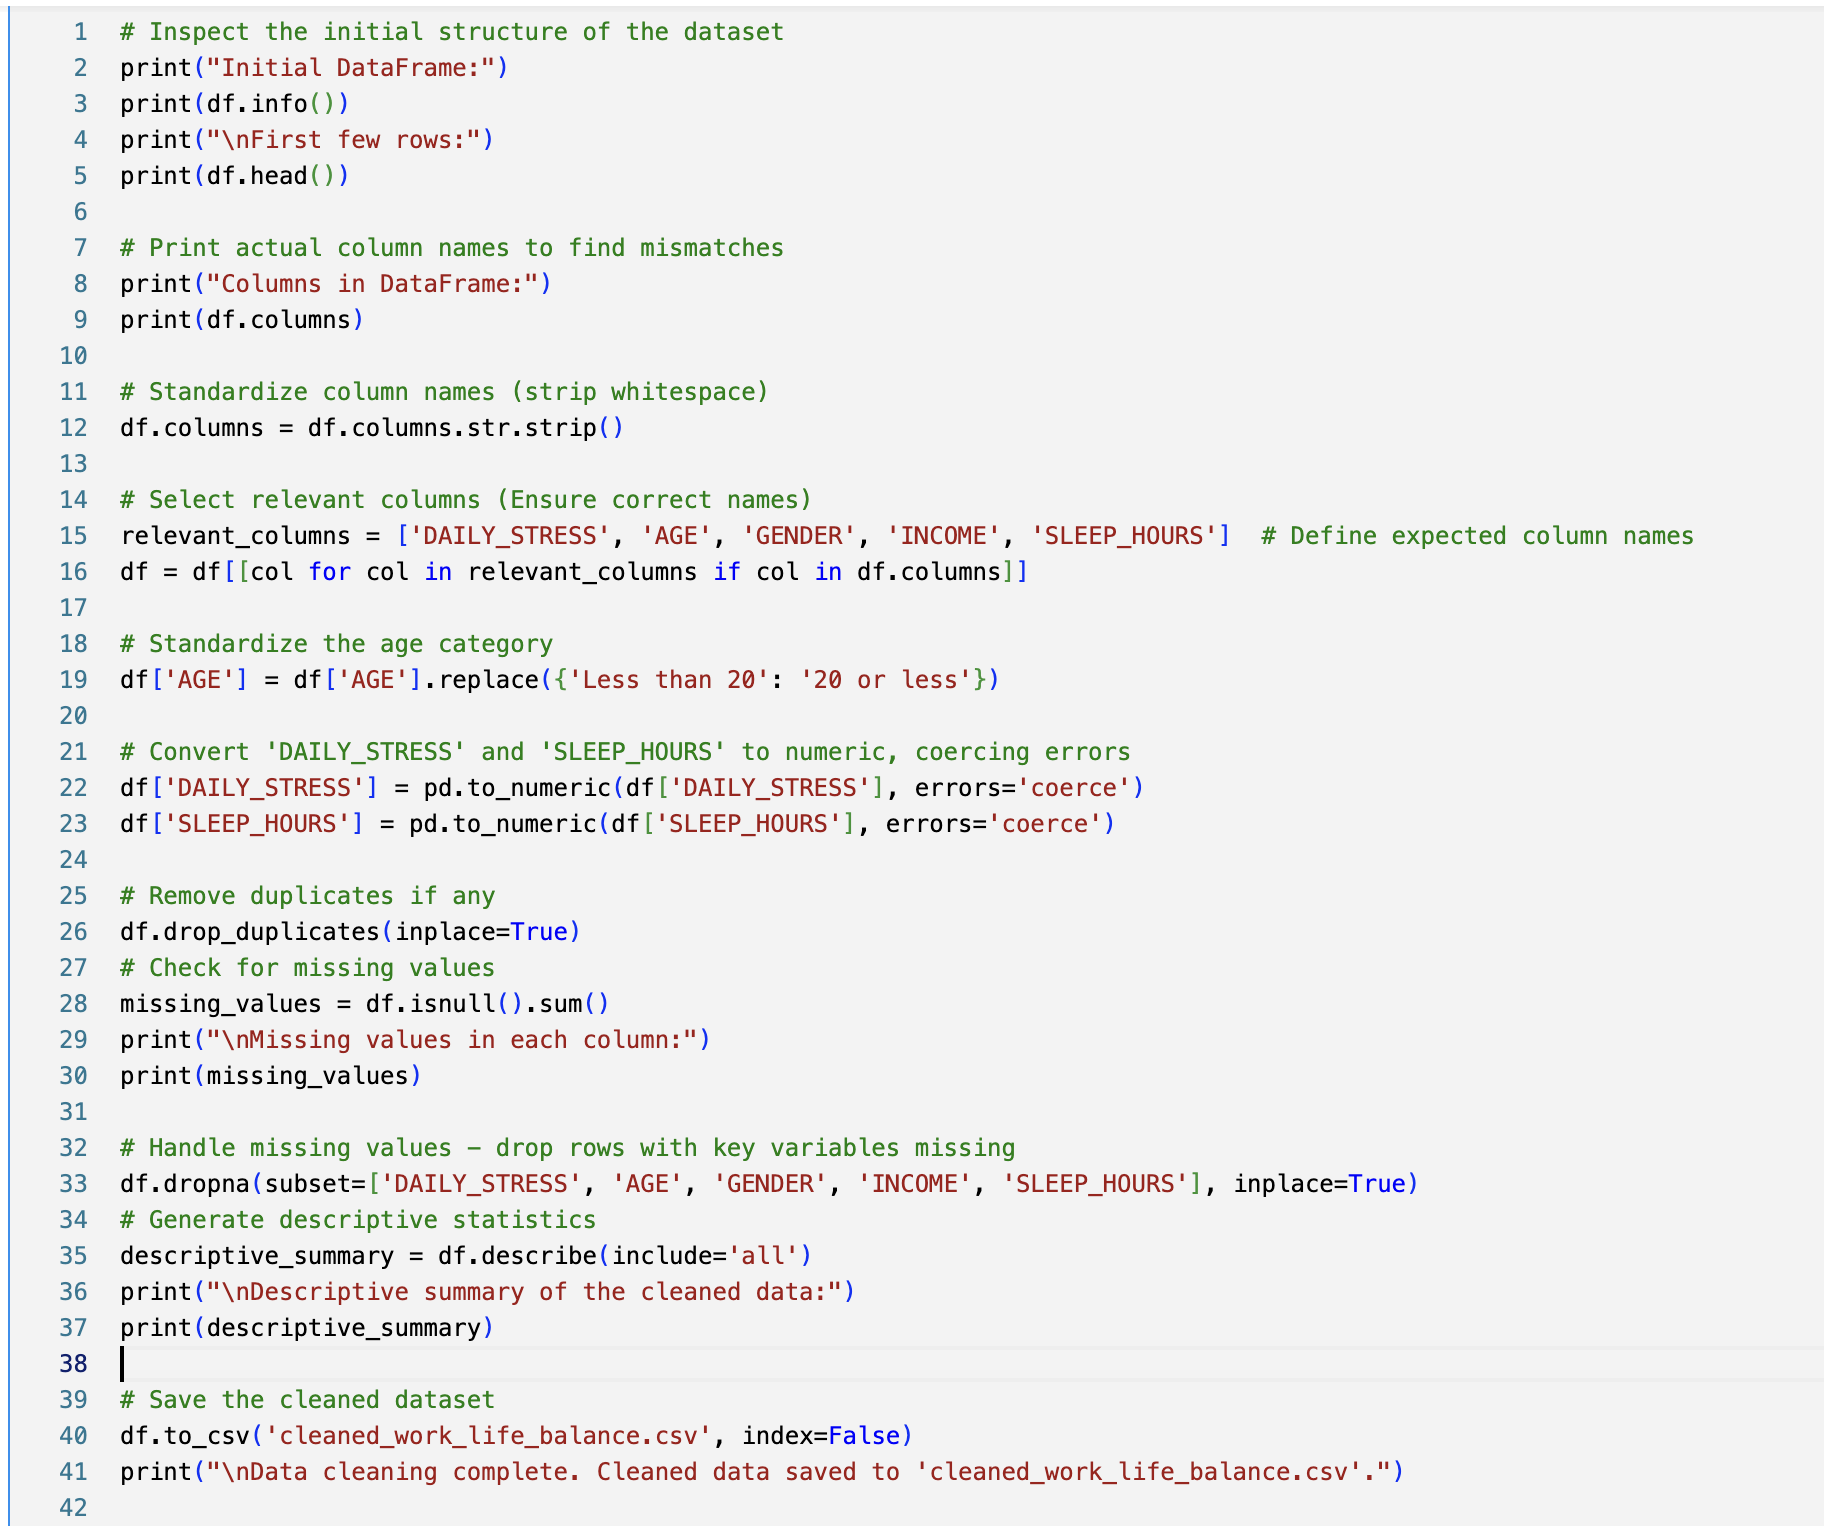
\includegraphics[width=1.2\linewidth]{CleaningCode1.png}
    \caption{Summary of cleaning code for Work-life Balance Survey} 
    \label{fig:enter-label}
\end{figure}

\clearpage
\begin{table}[ht]
    \centering
    \caption{Attributes, Descriptions, and Possible Values from Work-Life Balance Survey}
    \label{tab:work_life_balance_attributes}
    \begin{tabular}{|l|p{5cm}|p{4cm}|} 
        \hline
        \textbf{Attribute} & \textbf{Description} & \textbf{Possible Values} \\ 
        \hline
        \textbf{DAILY\_STRESS}      & Perceived daily stress level & Whole numbers (e.g., 1, 2, 3, 4, 5) \\ 
        \hline
        \textbf{AGE}                 & Age group of respondents & "20 or less", "21 to 35", "36 to 50", "51 or more" \\ 
        \hline
        \textbf{GENDER}              & Gender of respondents & "Male", "Female", "Other" \\ 
        \hline
        \textbf{SUFFICIENT\_INCOME}  & Indicates if the income is sufficient & 0 (No), 1 (Yes) \\ 
        \hline
        \textbf{SLEEP\_HOURS}        & Average hours of sleep per night & Whole numbers (e.g., 4, 5, 6, 7, 8, 9) \\ 
        \hline
    \end{tabular}
\end{table}


\subsection{Healthcare Dataset Stroke Data}

The data preprocessing workflow for the healthcare stroke dataset employs several key techniques to ensure the dataset is ready for analysis. Initially, the dataset is loaded using Pandas, and the first step involves examining its structure and identifying any missing values, which informs subsequent cleaning procedures. A selection of relevant features, including age, gender, hypertension status, heart disease, and more, is made to focus the analysis. To address missing values, categorical variables such as gender and marital status are encoded using LabelEncoder, converting them into a numerical format suitable for machine learning models. The K-nearest neighbors (KNN) imputation method is applied specifically to the body mass index (BMI) column, filling in gaps based on similar observations. The target variable, stroke status, is then transformed into a binary format for easier classification. After addressing missing values, a correlation analysis is conducted to explore relationships between variables, and the data is split into training and testing sets to enable robust model evaluation. To enhance model performance, feature scaling is performed using Min-Max scaling, ensuring all features are on a similar scale. Additionally, class imbalance in the target variable is addressed using the Synthetic Minority Over-sampling Technique (SMOTE), which balances the number of instances of each class in the training set. Finally, the cleaned and processed dataset is saved for future modeling efforts, completing a comprehensive cleaning and preprocessing pipeline that prepares the data for effective exploratory analysis and predictive modeling.

\subsubsection{Dataset Cleaning Code and Variable Attributes}

The following code and tables summarize the cleaned data attributes, including their descriptions, data types, and possible values.

\clearpage
\begin{figure}
    \centering
    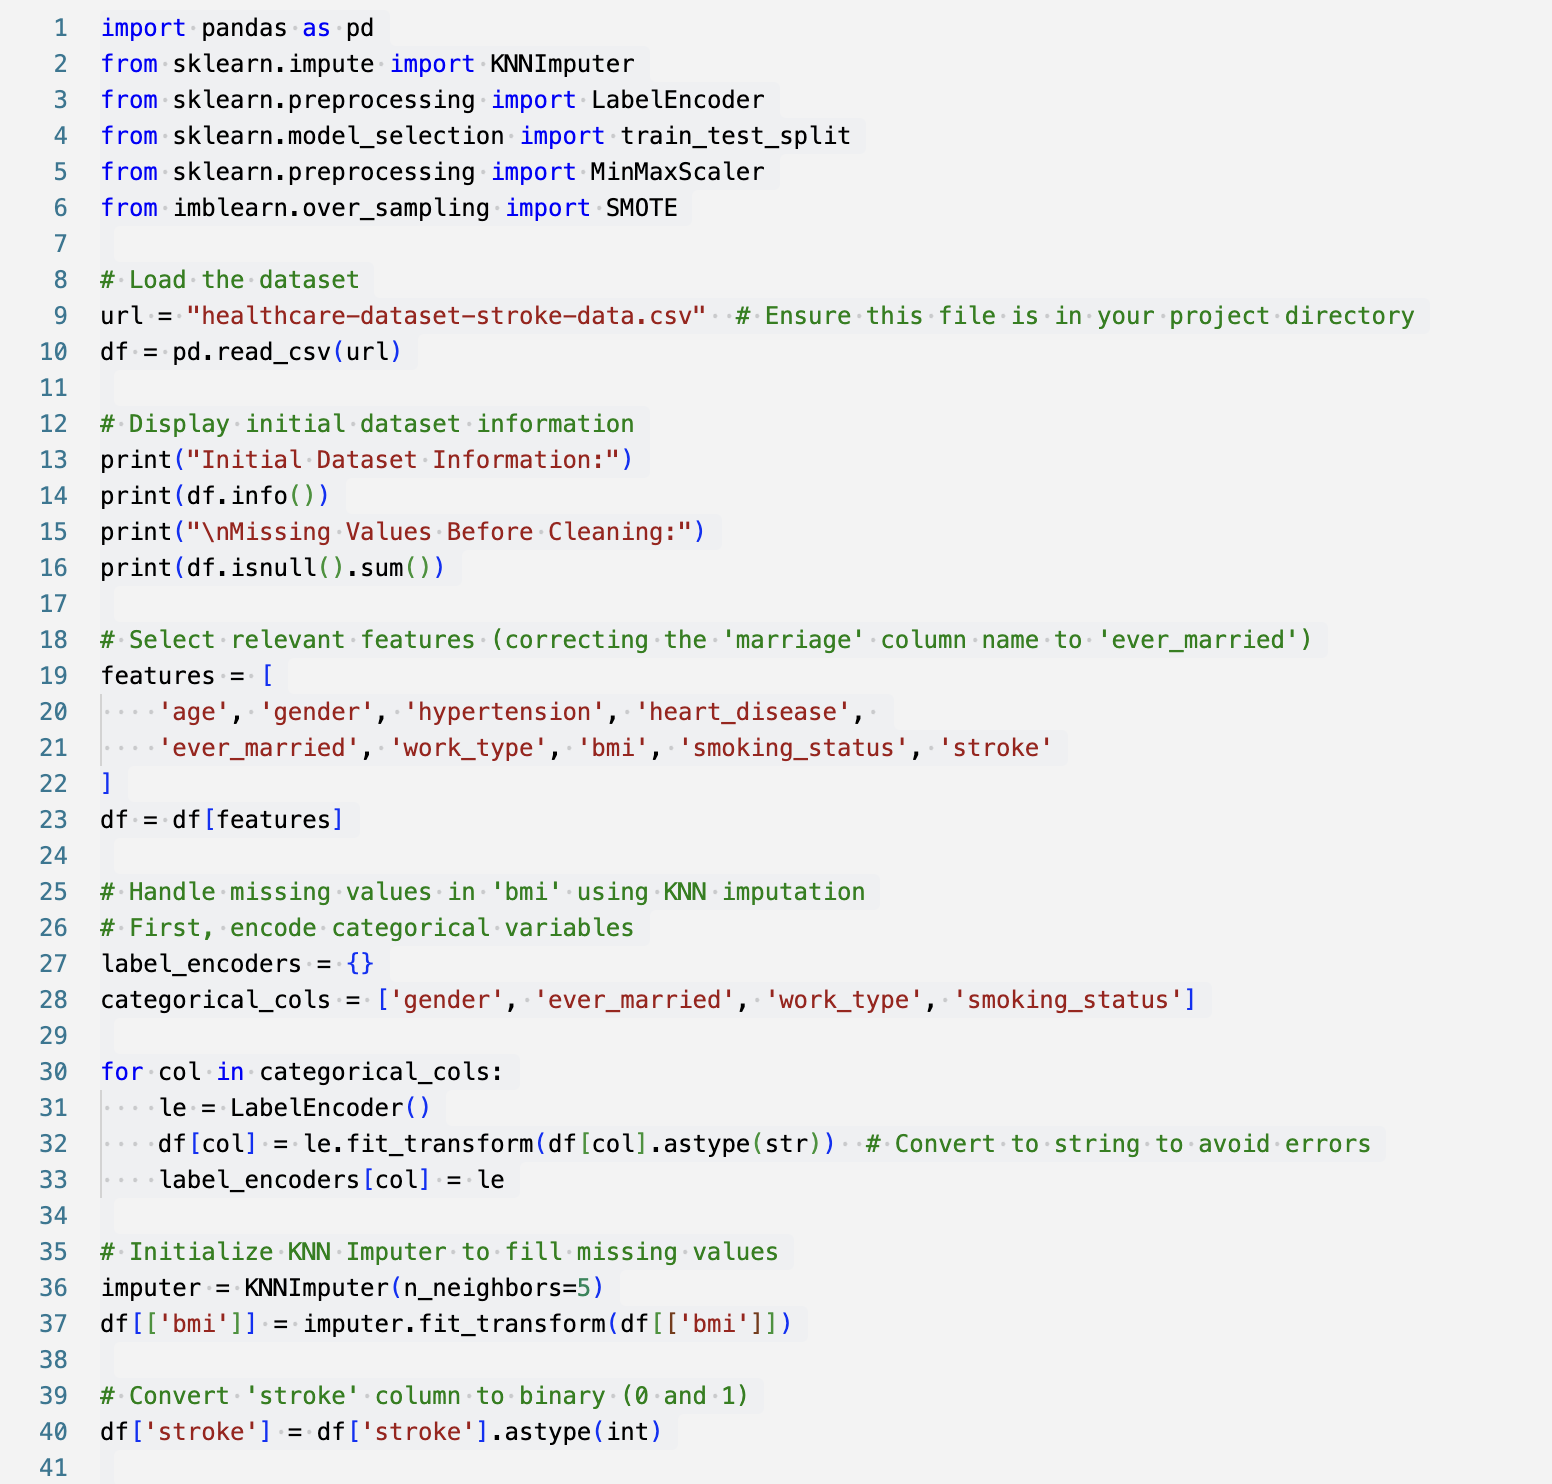
\includegraphics[width=.75\linewidth]{Cleaning1.png}
    \centering
    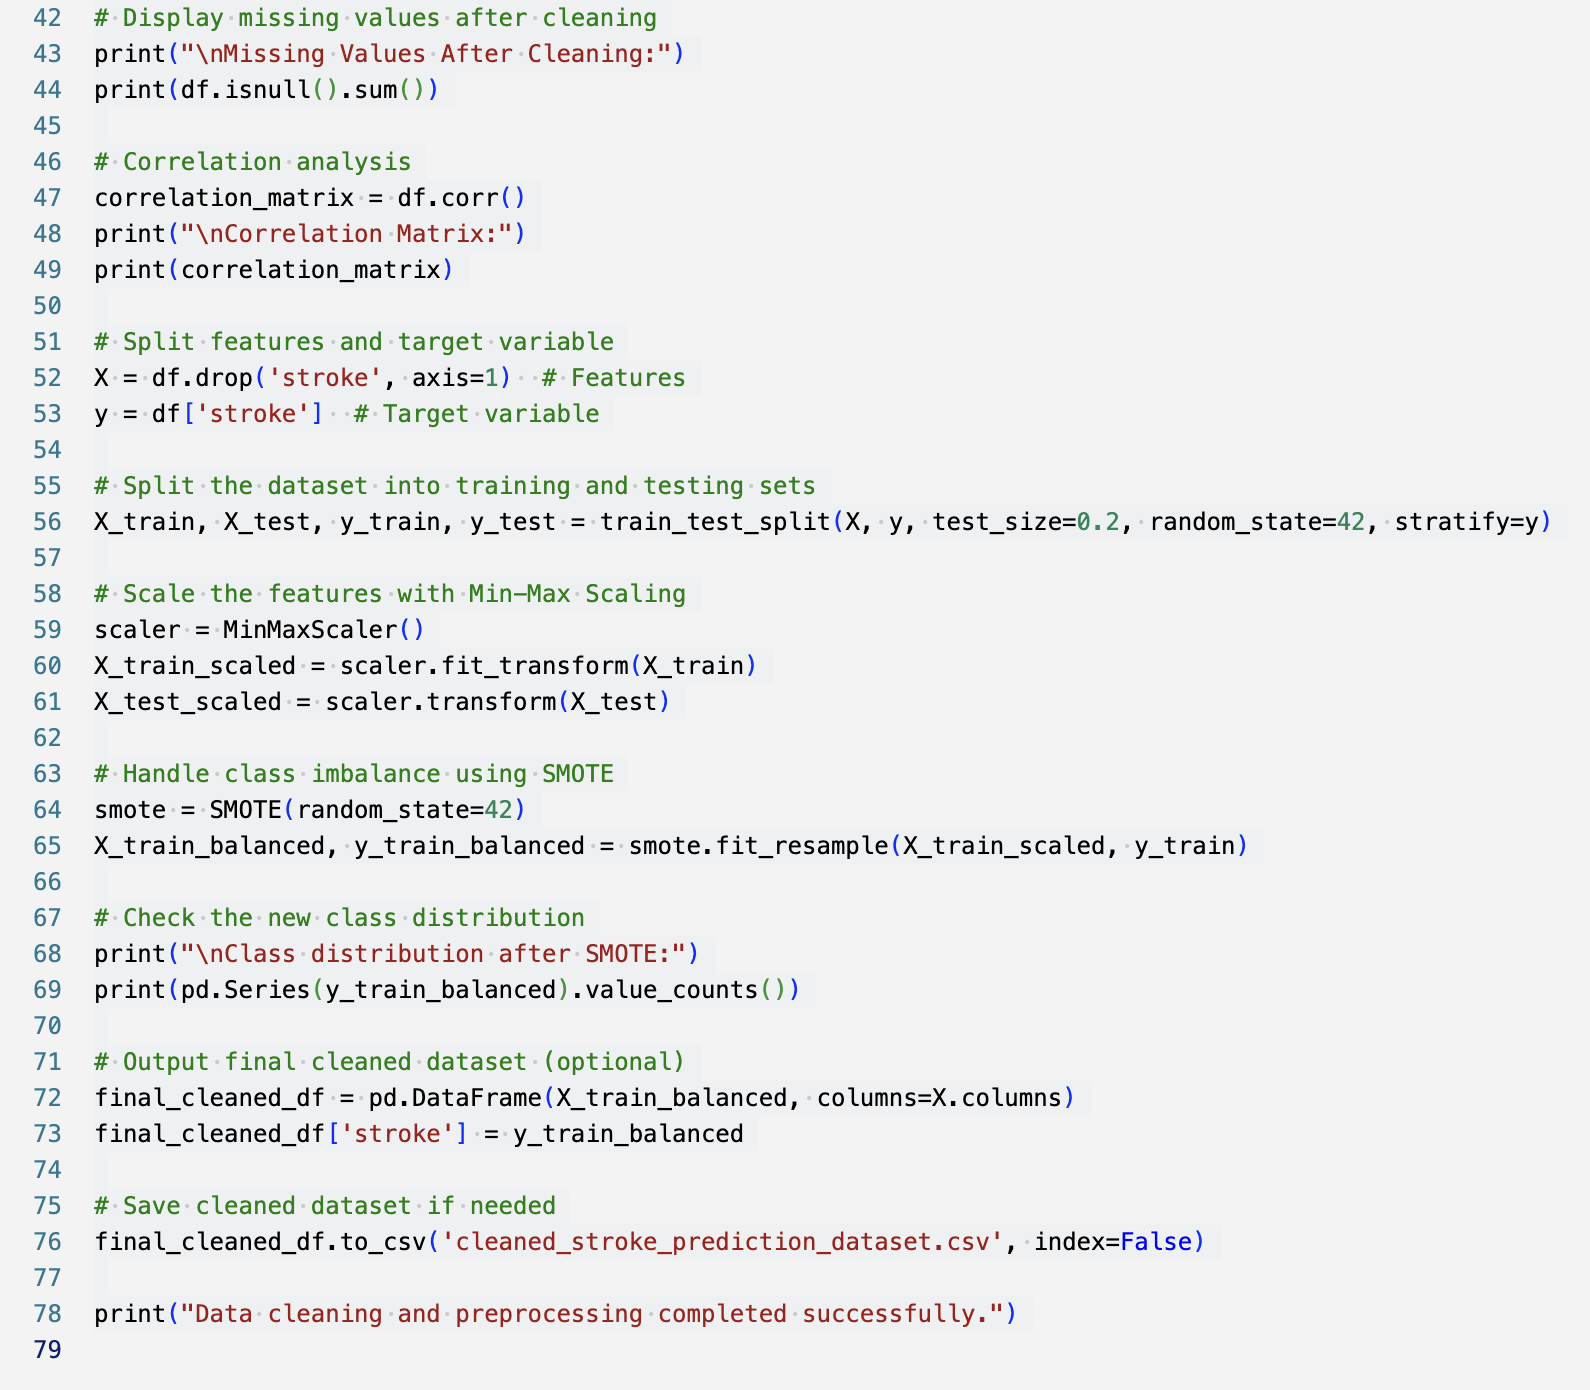
\includegraphics[width=.75\linewidth]{Cleaning2.png}
    \caption{Summary of cleaning code for Healthcare Dataset} 
    \label{fig:enter-label}
\end{figure}

\clearpage
\begin{table}[ht]
\centering    
\caption{Attributes, Descriptions, and Possible Values from Healthcare Dataset - Stroke Data} 
\label{tab1} 

\begin{tabular}{|l|p{5cm}|p{4cm}|} 
\hline     
\textbf{Attribute} & \textbf{Description} & \textbf{Possible Values} \\        
\hline        
\textbf{age} & Age of the patient in years & Whole numbers (e.g., 0, 1, 25, 60) \\        
\hline        
\textbf{gender} & Gender of the patient & "Male", "Female", "Other" \\        
\hline        
\textbf{hypertension} & Indicates if the patient has hypertension & 0 (No), 1 (Yes) \\        
\hline        
\textbf{heart\_disease} & Indicates if the patient has heart disease & 0 (No), 1 (Yes) \\        
\hline        
\textbf{ever\_married} & Indicates if the patient has ever been married & "No", "Yes" \\        
\hline        
\textbf{work\_type} & Type of employment of the patient & "Children", "Govt job", "Never worked", "Private", "Self-employed" \\        
\hline        
\textbf{bmi} & Body Mass Index of the patient & Positive floats (e.g., 18.5, 30.0) \\        
\hline        
\textbf{smoking\_status} & Indicates the smoking status of the patient & "Formerly smoked", "Smokes" \\        
\hline    
\end{tabular}    
\end{table}

\begin{table}[ht]
    \centering
    \begin{minipage}{0.45\linewidth}
        \centering
        \caption{Daily Stress Levels}\label{tab:stress_levels}
        \begin{tabular}{|l|l|}
            \hline
            \textbf{Stress Level (0-10)} & \textbf{Count} \\ 
            \hline
            0.00 - 0.25 & 676 \\ 
            1.00 - 1.25 & 2,478 \\ 
            2.00 - 2.25 & 3,407 \\ 
            3.00 - 3.25 & 4,398 \\ 
            4.00 - 4.25 & 2,960 \\ 
            4.75 - 5.00 & 2,052 \\ 
            \hline
        \end{tabular}
    \end{minipage}
    \hspace{0.05\linewidth} % Space between the tables
    \begin{minipage}{0.45\linewidth}
        \centering
        \caption{Typical Sleep Hours}\label{tab:sleep_hours}
        \begin{tabular}{|l|l|}
            \hline
            \textbf{Sleep Hours (0-10)} & \textbf{Count} \\ 
            \hline
            1.00 - 1.45 & 18 \\ 
            1.90 - 2.35 & 21 \\ 
            2.80 - 3.25 & 49 \\ 
            3.70 - 4.15 & 252 \\ 
            4.60 - 5.05 & 1,025 \\ 
            5.95 - 6.40 & 3,397 \\ 
            6.85 - 7.30 & 5,566 \\ 
            7.75 - 8.20 & 4,324 \\ 
            8.65 - 9.10 & 987 \\ 
            9.55 - 10.00 & 333 \\ 
            \hline
        \end{tabular}
    \end{minipage}
\end{table}


\clearpage

\begin{table}[ht]
    \centering
    
    \begin{minipage}{0.45\linewidth}
        \centering
        \caption{Income Sufficiency}\label{tab:income_sufficiency}
        \begin{tabular}{|l|l|}
            \hline
            \textbf{Income Sufficiency} & \textbf{Count} \\ 
            \hline
            1.00 - 1.05 & 4,329 \\ 
            1.95 - 2.00 & 11,643 \\ 
            \hline
        \end{tabular}
    \end{minipage}
    \hspace{0.05\linewidth} % Space between the tables
    \begin{minipage}{0.45\linewidth}
        \centering
        \caption{Demographic Breakdown}\label{tab:demographic_breakdown}
        \begin{tabular}{|l|l|}
            \hline
            \textbf{Age Group} & \textbf{Percentage} \\ 
            \hline
            21 to 35 & 38\% \\ 
            36 to 50 & 29\% \\ 
            Other & 33\% \\ 
            \hline
        \end{tabular}
    \end{minipage}
    \hspace{0.05\linewidth} % Space between the tables
    \begin{minipage}{0.45\linewidth}
        \centering
        \caption{Gender Breakdown}\label{tab:gender_breakdown}
        \begin{tabular}{|l|l|}
            \hline
            \textbf{Gender} & \textbf{Percentage} \\ 
            \hline
            Female & 62\% \\ 
            Male & 38\% \\ 
            \hline
        \end{tabular}
    \end{minipage}
\end{table}

\section{Exploratory Data Analysis}




\clearpage
\begin{figure}
    \centering
    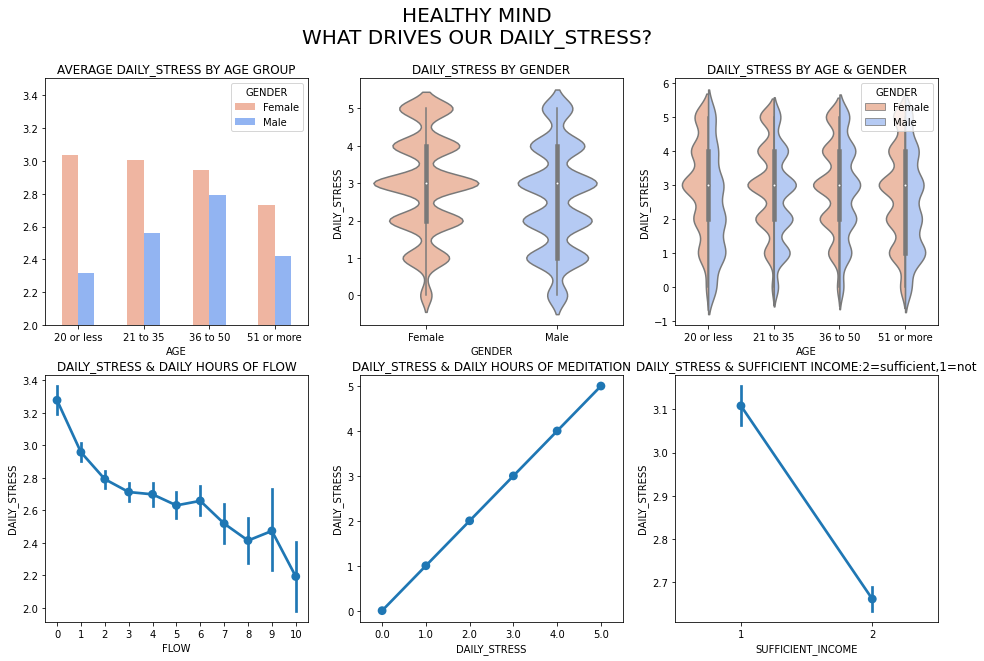
\includegraphics[width=1.2\linewidth]{__results___16_0.png}
    \caption{Summary of Daily Stress}\cite{Work-Life}
    \label{fig:enter-label}
\end{figure}


\clearpage
\nocite{*}
\bibliographystyle{splncs04}
\bibliography{mybibliography}


%


\end{document}
